\chapter*{Аннотация}		% Заголовок
\addcontentsline{toc}{chapter}{Аннотация}	% Добавляем его в оглавление

В данной работы мы сделали то и это. Использовали Coq, красили графы, веселились.

\chapter*{Введение}		% Заголовок
\addcontentsline{toc}{chapter}{Введение}	% Добавляем его в оглавление

\section{Хроматическое число плоскости. Задача Нелсона — Эрдёша — Хадвигера}

Граф $G$ -- это упорядоченная пара $G := (V, E)$, где $V$ -— непустое множество, а $E$ — подмножество $V\times V$. Если $(u, v) \in E$, то вершины $u$ и $v$ называются { \it смежными}. Обозначение $u \sim v$.

Раскраска $f$ графа $G$ -- это отображение из $V$ в множество цветов. 
Раскраска $f$ называется {\it правильной}, если $u \sim v \rightarrow f(u) \neq  f(v)$

{\it Хроматическое число} графа --- это минимальное количество цветов, в которые можно правильно раскрасить граф.

{\it Граф единичных расстояний} -- это граф, вершинами которого являются некоторые точки евклидовой плоскости, а ребрами соединены все пары вершин,  находящиеся на расстоянии $1$.

{\it Хроматическое число плоскости $\chi$ } --- это минимальное число цветов $\chi$, в которое можно правильно раскрасить любой граф единичных расстояний.

Задача Нелсона — Эрдёша — Хадвигера заключается в нахождении хроматического числа плоскости. C 1950 года известно \cite{Soi}, что хроматическое число плоскости хотя бы 4 и не больше 7. 

\textbold{TODO:} объяснить, почему, прикрепить картинки про 4 и 7, \cite{Had}.

\begin{figure}[ht] 
  \center
  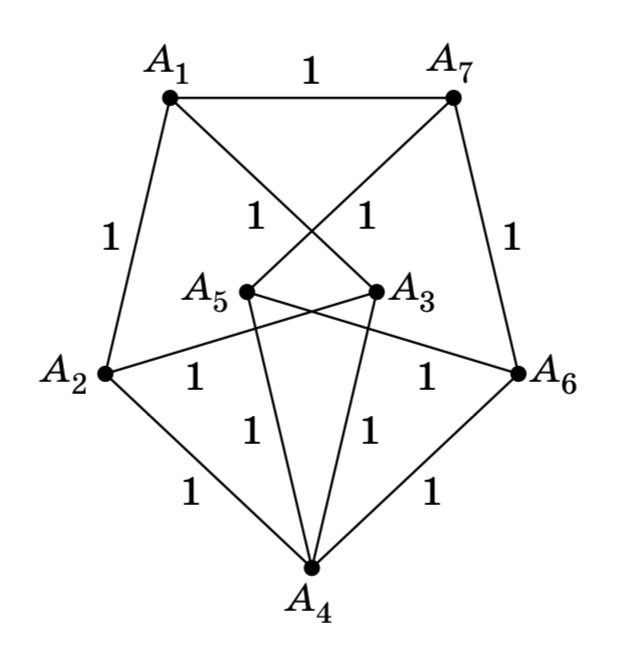
\includegraphics [width=0.8\linewidth] {Moser_Spindle}
  \caption{Веретено Мозера} 
  \label{img:latex}
\end{figure}

\begin{figure}[ht] 
  \center
  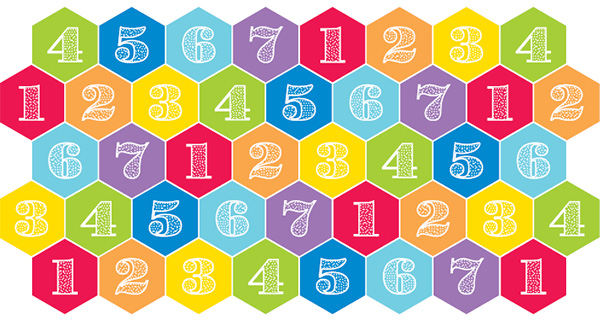
\includegraphics [width=0.8\linewidth] {raskraska7}
  \caption{Раскраска плоскости в 7 цветов} 
  \label{img:latex}
\end{figure}

В апреле 2018 года Обри де Грей опубликовал статью, в которой доказал, что хроматическое число плоскости хотя бы 5. На момент написания работы задача является открытой. Данная работа фокусируется на уточнении неясных мест в данной статье, явных детерминированных конструкциях графов из статьи и верификации отдельных утверждений статьи в системе Coq.

\section{Система Coq. Описание, история, возможности, применения}
История создания, история использования (сортировки, раскраска карты, \cite{} что-нибудь.)

Какая логика? Че за изоморфизм там? Что такое Галина? Мы пользуемся Галиной? Что такое тактики?

Мы будем пользоваться представлением графа чувака автора учебника, \cite{} учебник.

\section{Мотивировка задачи} \label{sect1_2}

Краткое изложение структуры статьи де Грея, статья просится на верификацию.


\section{Обзор литературы}

1. Huele
2. Exoo, Geoffrey; Ismailescu, Dan 

Пацаны проверили на SAT solver-e, кто-то придумал пример поменьше, кто-то графы по-другому делает.


\newcommand{\actuality}{}

%% регистрируем счётчики в системе totcounter
\regtotcounter{totalcount@figure}
\regtotcounter{totalcount@table}       % Если поставить в преамбуле то ошибка в числе таблиц
\regtotcounter{TotPages}               % Если поставить в преамбуле то ошибка в числе страниц

% \textbf{Объем и структура работы.} Работа состоит из~введения, трёх глав, заключения и~двух приложений.
%% на случай ошибок оставляю исходный кусок на месте, закомментированным
%Полный объём диссертации составляет  \ref*{TotPages}~страницу с~\totalfigures{}~рисунками и~\totaltables{}~таблицами. Список литературы содержит \total{citenum}~наименований.
%
% Полный объём работы составляет \formbytotal{TotPages}{страниц}{у}{ы}{} 
% с~\formbytotal{totalcount@figure}{рисунк}{ом}{ами}{ами}
% и~\formbytotal{totalcount@table}{таблиц}{ей}{ами}{ами}. Список литературы содержит  
% \formbytotal{citenum}{наименован}{ие}{ия}{ий}.
